% 
% Lecture Template for ME3023 -  Measurements in Mechanical Systems - Tennessee Technological University
%
% Spring 2020 - Summer 2020
% Tristan Hill, May 07, 2020 - June 12, 2020
% Module 5 - Strain Applications
% Topic 2 - Apparent Strain
%

%\documentclass{beamer}                         % for presentation (has nav buttons at bottom)
\documentclass[handout]{beamer}  % for handout 
\usepackage{beamerthemesplit}
\usepackage{amsmath}
\usepackage{listings}
\usepackage{multicol}
\usepackage{framed}

\beamertemplateballitem

% custom colors
\definecolor{TTUpurple}{rgb}{0.3098, 0.1607, 0.5176} % TTU Purple (primary)
\definecolor{TTUgold}{rgb}{1.0000, 0.8666, 0.0000} % TTU Gold (primary) 
\definecolor{mygray}{rgb}{.6, .6, .6}
\definecolor{mypurple}{rgb}{0.6,0.1961,0.8}
\definecolor{mybrown}{rgb}{0.5451,0.2706,0.0745}
\definecolor{mygreen}{rgb}{0, .39, 0}
\definecolor{mypink}{rgb}{0.9960, 0, 0.9960}

% color commands
\newcommand{\R}{\color{red}}
\newcommand{\B}{\color{blue}}
\newcommand{\BR}{\color{mybrown}}
\newcommand{\K}{\color{black}}
\newcommand{\G}{\color{mygreen}}
\newcommand{\PR}{\color{mypurple}}
\newcommand{\PN}{\color{mypink}}
\newcommand{\OR}{\color{TTU}}
\newcommand{\GD}{\color{TTUgold}}


\setbeamercolor{palette primary}{bg=TTUpurple,fg=TTUgold}
\setbeamercolor{palette secondary}{bg=black,fg=TTUgold}
\setbeamercolor{palette tertiary}{bg=black,fg=TTUpurple}
\setbeamercolor{palette quaternary}{bg=TTUgold,fg=black}
\setbeamercolor{structure}{fg=TTUpurple} % itemize, enumerate, etc
\setbeamercolor{section in toc}{fg=TTUpurple} % TOC sections

%\usefonttheme{professionalfonts}

\newcommand{\Lagr}{\mathcal{L}} % lagrangian

\newcommand{\hspcu}{\underline{\hspace{20mm}}} % large horizontal space w underline
\newcommand{\vspccc}{\vspace{6mm}\\} % large vertical space
\newcommand{\vspcc}{\vspace{4mm}\\}   % medium vertical space
\newcommand{\vspc}{\vspace{2mm}\\}     % small vertical space

\newcommand{\hspcccc}{\hspace{10mm}} % large horizontal space
\newcommand{\hspccc}{\hspace{6mm}} % large horizontal space
\newcommand{\hspcc}{\hspace{4mm}}   % medium horizontal space
\newcommand{\hspc}{\hspace{2mm}}     % small horizontal space

\newcommand{\eqscl}{0.9}     % small horizontal space


\author{ME3023 - Measurements in Mechanical Systems} % original formatting from Mike Renfro, September 21, 2004

\newcommand{\MNUM}{5\hspace{2mm}} % Module number
\newcommand{\TNUM}{2\hspace{2mm}} % Topic number 
\newcommand{\moduletitle}{Strain Applications}
\newcommand{\topictitle}{Multiple Gauge Bridge} 

\newcommand{\sectiontitleI}{The Quarter Bridge}
\newcommand{\sectiontitleII}{Using Multiple Gauges}
\newcommand{\sectiontitleIII}{Apparent Strain and Temperature}
\newcommand{\sectiontitleIV}{Example: Digital Scale}

% custom box
\newsavebox{\mybox}

\title{Module \MNUM - \moduletitle}

\date{Mechanical Engineering\vspc Tennessee Technological University}

\begin{document}

\lstset{language=MATLAB,basicstyle=\ttfamily\small,showstringspaces=false}

\frame{\titlepage \center\begin{framed}\Large \textbf{Topic \TNUM - \topictitle}\end{framed} \vspace{5mm}}

% Section 0: Outline
\frame{

\large \textbf{Topic \TNUM - \topictitle} \vspace{3mm}\\

\begin{itemize}

	\item \sectiontitleI		\vspc % Section I
	\item \sectiontitleII 	\vspc % Section II
	\item \sectiontitleIII 	\vspc %Section III
	\item \sectiontitleIV 	\vspc %Section IV

\end{itemize}

}

% Section I:
\section{\sectiontitleI}

% Section I - Frame I:
\frame{
\frametitle{\sectiontitleI}
\small

Hooke's law describes the linear relationship between stress and strain of an elastic member with modulus of elasticity E.\vspc
\scalebox{1}{$\sigma=E\epsilon$} \vspc
\begin{multicols}{2}
If the loading is known the beam models can be applied. \vspc
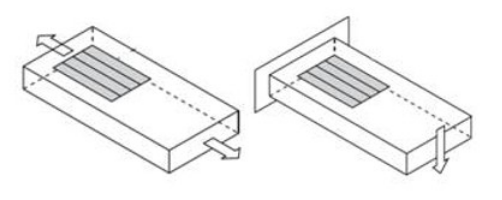
\includegraphics[scale=.30]{simple_loading.png} 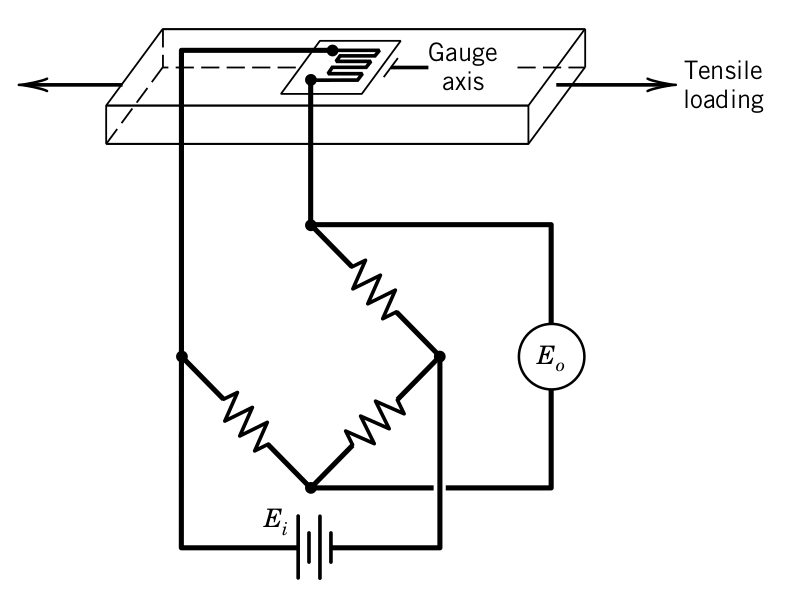
\includegraphics[scale=.18]{gauged_beam_bridge.png} \vspace{15mm} 
\end{multicols}

}

% Section I - Frame II:
\frame{
\frametitle{\sectiontitleI}
\small
\begin{multicols}{2}
Consider the quarter bridge case in which the gauge is $R_1$ and $R_1=R_2=R_3=R_4$ in a condition of zero strain. \vspcc

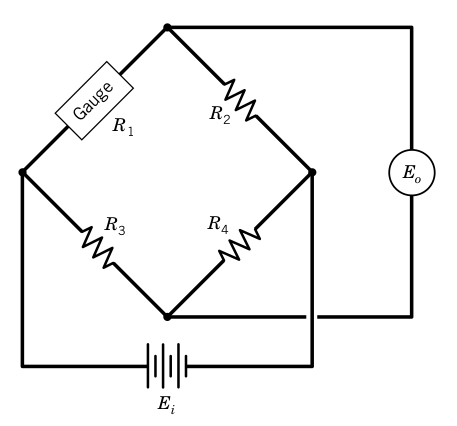
\includegraphics[scale=.18]{bridge_circuit_fig2.png}
\end{multicols}

\scalebox{1}{$E_{out}=E_{in}\times\left( \frac{R_1}{R_1+R_2}-\frac{R_3}{R_3+R_4}\right)\implies E_{out}=E_{in}\frac{\left(R_1R_4-R_2R_3\right)}{\left(R_1+R_2\right)\left(R_3+R_4\right)}$}\vspcc
Now, $R_1$ changes by $\delta R$ causing $E_{out}$ to change by $\delta E_{out}$. \vspcc
\scalebox{1}{$E_{out}+\delta E_{out}=E_{in}\frac{\left(\left(R_1+\delta R\right)R_4-R_2R_3\right)}{\left(\left(R_1+\delta R\right)+R_2\right)\left(R_3+R_4\right)}$}\vspc

}

% Section I - Frame III:
\frame{
\frametitle{\sectiontitleI}
\small

In practice the bridge is balanced in a condition of zero strain which gives an output voltage of $E_{out}=0v$. Then any additional strain causes a $\delta E_{out}$ which is measured. \vspc

The previous equation is commonly written in the following practical form. \vspcc

\scalebox{1}{$\frac{\delta E_{out}}{E_{in}}=\frac{\delta R/R}{4+2\left(\delta R/R\right)}\approx \frac{\delta R/R}{4}$} \hspc or \hspc \scalebox{1}{$\frac{\delta E_{out}}{E_{in}}=\frac{GF\epsilon}{4+2GF\epsilon}\approx \frac{ GF\epsilon}{4}$} \vspcc
with Gage Factor defined as \hspc \scalebox{1}{$GF\equiv \frac{\delta R/R}{\delta L/L}=\frac{\delta R/R}{\epsilon}$}

}


% Section II:
\section{\sectiontitleII}

% Section II - Frame I:
\frame{
\frametitle{\sectiontitleII}
\small
An improved system uses a set of gauges known as a {\PN rosette} with the wheatstone bridge in a half or full bridge configuration. \vspc

\begin{multicols}{2}
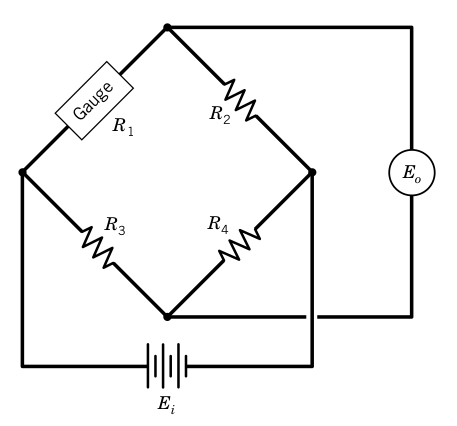
\includegraphics[scale=.2]{bridge_circuit_fig2.png}

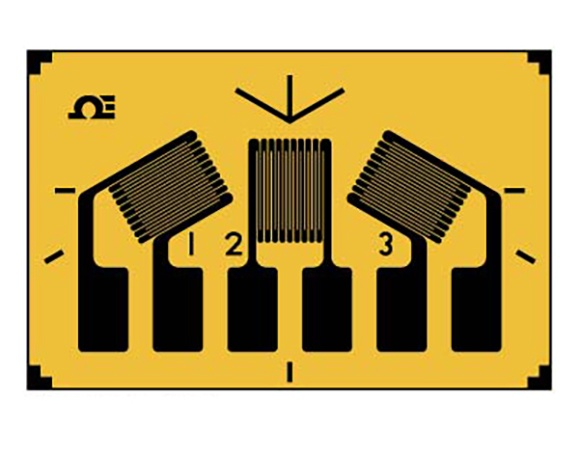
\includegraphics[scale=.2]{delta_rosette.jpg}
\end{multicols}
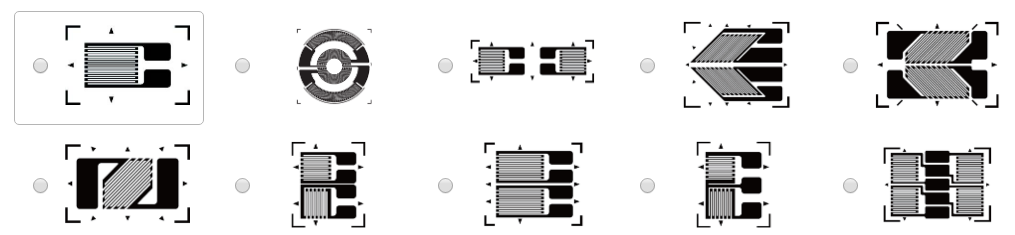
\includegraphics[scale=.4]{gauge_geometries.png}

}
% Section II - Frame II:
\frame{
\frametitle{\sectiontitleII}
\begin{multicols}{2}
If multiple gauges are used the relationship between strain and output voltage is derived with a similar process (see page 479).   \vspcc

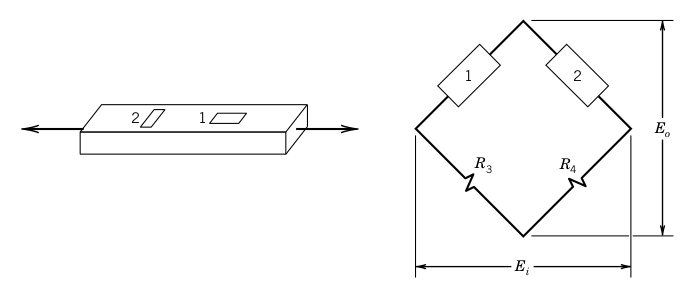
\includegraphics[scale=.2]{half_bridge_beam.png}
\end{multicols}

The result gives an expression relating the output voltage, the gauge factor, and all four measured strains. \vspcc

\scalebox{1}{$\frac{\delta E_{out}}{E_{in}}=\frac{GF}{4}\left(\epsilon_1-\epsilon_2+\epsilon_4-\epsilon_3\right)$}\vspcc

%The constant $\kappa$ is known as the bridge constant.

}


% Section III:
\section{\sectiontitleIII}

% Section III - Frame I:
\frame{
\frametitle{\sectiontitleIII}
Equation 11.22 shows that for a bridge containing one or more strain gauges, equal strains on opposite bridge arms sum, whereas equal strains on adjacent arms of the bridge cancel. These characteristics can be used to increase the output of the bridge, to provide temperature compensation, or to cancel unwanted components of strain. \vspc

{\tiny Text: Theory and Design of Mechanical Measurements} \vspcc

This summarizes the reasons to use a wheatstone instead of a operational amplifier when measuring strain with a metallic strain gauge. 

}

% Section III - Frame II:
\frame{
\frametitle{\sectiontitleIII}
\small

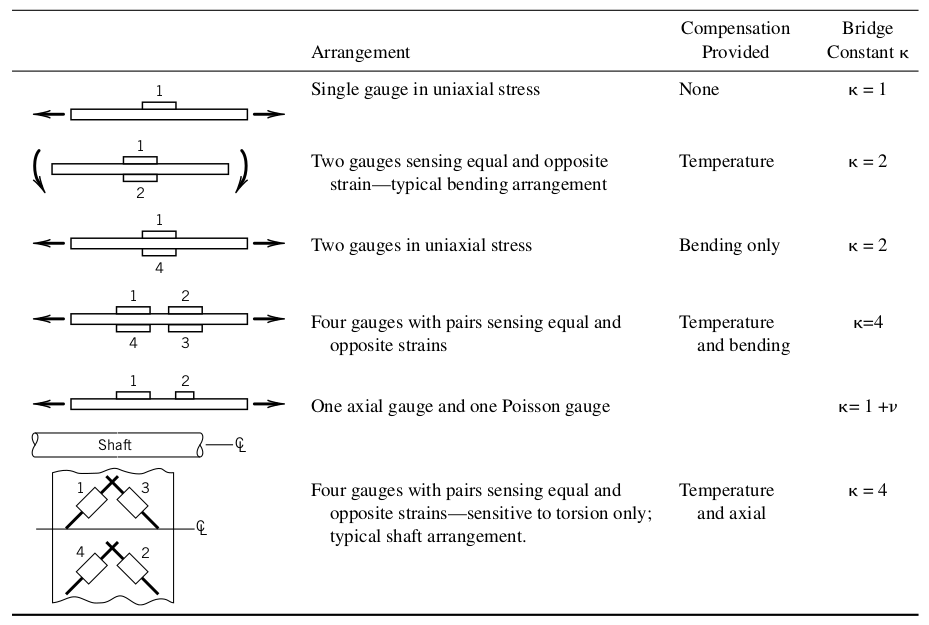
\includegraphics[scale=.28]{gauge_configurations.png}\\
For more details read this document from \href{https://www.ni.com/en-us/innovations/white-papers/07/measuring-strain-with-strain-gages.html}{NI}.
}

% Section IV:
\section{\sectiontitleIV}

% Section IV - Frame I:
\frame{
\frametitle{\sectiontitleIV}

\begin{multicols}{2}
Have you ever wondered how a digital scale works? \vspcc

Does it matter where you place item? Why or why not?

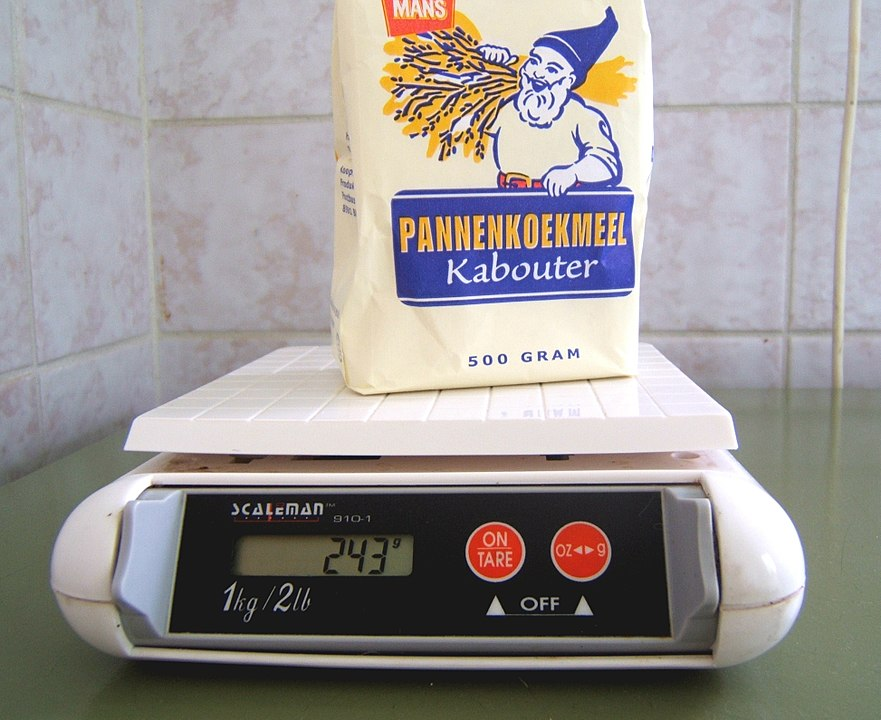
\includegraphics[scale=.2]{digital_scale.jpg}
\end{multicols}

}
	
\end{document}





